\subsection{Convergenza}

Per discutere l'\textbf{accuratezza della soluzione numerica} trovata da ciascun metodo introdotto per determinati valori di $h$, è necessario introdurre la definizione di \textbf{convergenza}:
\begin{equation}\label{eq: convergenza}
	\left|y\left(t_{n}\right) - u_{n}\right| = O\left(h\right) \hspace{2em} n = 0, \dots, N
\end{equation}
\begin{figure}[!htp]
	\centering
	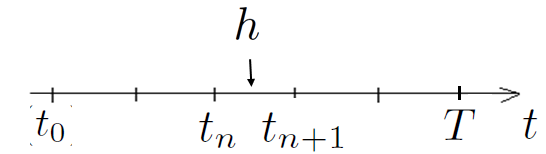
\includegraphics[width=.4\textwidth]{img/convergenza-1.png}
\end{figure}

\noindent
Modificando la convergenza appena introdotta (eq. \ref{eq: convergenza}), essa rappresenta la \textbf{stima dell'errore di convergenza}:
\begin{equation}
	\left|y\left(t_{n}\right) - u_{n}\right| = O\left(h^{p}\right) \hspace{2em} n = 0, \dots, N
\end{equation}
Inoltre si dice che il \textbf{metodo numerico è di ordine $p$}. È interessante notare che all'\textbf{aumentare di $p$}, la \textbf{velocità di convergenza aumenta}.

\highspace
Utilizzando $\lambda$ del coefficiente del \emph{problema modello lineare}, oppure:
\begin{equation*}
	\overline{\lambda} = -\underset{t,y}{\max} \left|\dfrac{\partial f}{\partial y}\right| \hspace{2em} \text{con } \dfrac{\partial f}{\partial y} < 0
\end{equation*}
Nella tabella \ref{table: convergenza e stabilità} sono riassunti i metodi introdotti in questo capitolo.

\begin{table}[!htp]
	\centering
	\begin{tabular}{@{} c c c c @{}}
		\toprule
		\textbf{Metodo} & \textbf{Espl./Impl.} & \textbf{Convergenza} & \textbf{Assoluta stabilità} \\
		\midrule
		Eulero in avanti & Esplicito & $O\left(h\right)$ & $h < -\dfrac{2}{\lambda}$ \\
		\cmidrule{1-4}
		Eulero all'indietro & Implicito & $O\left(h\right)$ & Sempre garantita \\
		\cmidrule{1-4}
		Crank-Nicolson & Implicito & $O\left(h^{2}\right)$ & Sempre garantita \\
		\cmidrule{1-4}
		Heun & Esplicito & $O\left(h^{2}\right)$ & $h < -\dfrac{2}{\lambda}$ \\
		\bottomrule
	\end{tabular}
	\caption{Proprietà di convergenza e stabilità dei metodi per approssimare le ODE.}
	\label{table: convergenza e stabilità}
\end{table}

\newpage

\subsubsection{Consistenza dei metodi di Eulero}

Innanzitutto si introduce l'\definition{errore di troncamento locale $\tau_{n}$}, il quale si \textbf{commette introducendo la soluzione esatta} $y$ nello schema numerico. Per il \textbf{metodo di Eulero in avanti} si ha:
\begin{equation}
	\tau_{n} = \left|f\left(t_{n}, y\left(t_{n}\right)\right) - \dfrac{y\left(t_{n+1}\right)-y\left(t_{n}\right)}{h}\right|
\end{equation}
E per il \textbf{metodo di Eulero all'indietro} si ha:
\begin{equation}
	\tau_{n} = \left|f\left(t_{n+1}, y\left(t_{n+1}\right)\right) - \dfrac{y\left(t_{n+1}\right)-y\left(t_{n}\right)}{h}\right|
\end{equation}

\highspace
Un metodo numerico è \definition{consistente} se vale:
\begin{equation}
	\lim\limits_{h \rightarrow 0} \tau_{n} = 0 \hspace{2em} \forall n
\end{equation}
Inoltre, se vale:
\begin{equation}
	\tau_{n} = O\left(h^{p}\right) \hspace{2em} \forall n
\end{equation}
Si dice che l'\textbf{ordine di consistenza è $p$}. Riguardo i \textbf{\emph{metodi di Eulero}}, essi sono \textbf{consistenti del primo ordine}.

\highspace
Si noti che l'\textbf{errore di troncamento locale} $\tau_{n}$ non è l'errore necessario per verificare la convergenza: $\left|y\left(t_{n}\right) - u_{n}\right|$. L'errore:
\begin{equation*}
	e_{n} = \left|y\left(t_{n}\right) - u_{n}\right|
\end{equation*}
È dato da due contributi:
\begin{itemize}
	\item L'\textbf{errore} $e_{n}^{1}$ è \textbf{dovuto localmente al metodo numerico}, ottenuto partendo dalla vera soluzione $y\left(t_{n-1}\right)$.
	
	\item L'\textbf{errore} $e_{n}^{2}$ è \textbf{dovuto alla \emph{propagazione degli errori}} commessi agli istanti precedenti
\end{itemize}
\begin{figure}[!htp]
	\centering
	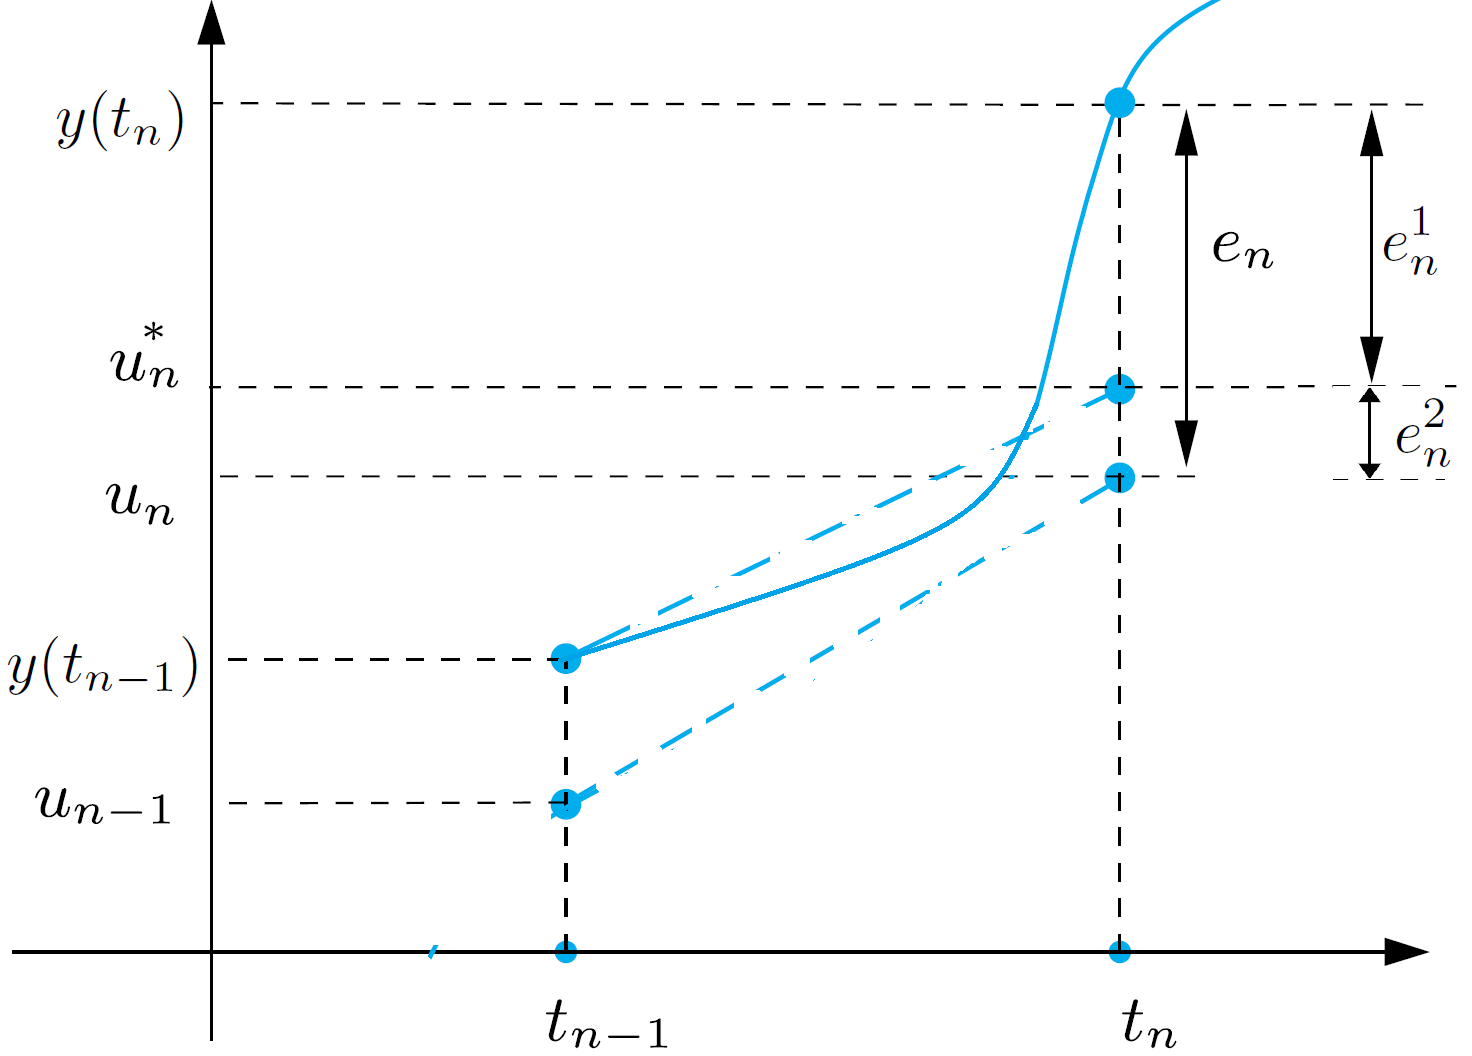
\includegraphics[width=.6\textwidth]{img/convergenza-2.png}
\end{figure}

\newpage

\noindent
Riguardo al \textbf{metodo di Eulero in avanti} l'\textbf{errore} è dato da:
\begin{itemize}
	\item Primo contributo dovuto localmente al metodo numerico:
	\begin{equation}
		e_{n}^{1} = \left|y\left(t_{n}\right) - y\left(t_{n-1}\right) - hf\left(t_{n-1}, y\left(t_{n-1}\right)\right)\right| = h\tau_{n-1}
	\end{equation}
	Da notare che il primo errore, a meno di un fattore $h$, è dato dall'errore di troncamento locale. Questo evidenzia come la \textbf{consistenza da sola non basti per avere la convergenza}.
	
	\item Secondo contributo dovuto alla propagazione degli errori:
	\begin{equation}
		e_{n}^{*} = \left|u_{n}^{*} - u_{n}\right|
	\end{equation}
\end{itemize}
Supponendo che valga la \textbf{condizione di assoluta stabilità} con $\overline{\lambda} = -\lambda_{\max}$:
\begin{equation*}
	h < \dfrac{2}{\lambda_{\max}}
\end{equation*}
Dunque si ha:
\begin{equation}
	\begin{array}{c}
		\left|e_{n}\right| \le \left|e_{n}^{1}\right| + \left|e_{n}^{2}\right| \le h\tau_{n-1} + \left|e_{n-1}\right| \\ [.5em]
		\downarrow \\ [.5em]
		\left|e_{n}\right| \le n h O\left(h\right) = \left(t_{n} - t_{0}\right)O\left(h\right)
	\end{array}
\end{equation}
Il \textbf{metodo di Eulero in avanti} è dunque \textbf{convergente} e del \textbf{primo ordine}. Lo stesso risultato vale anche per il \textbf{metodo di Eulero all'indietro}. In generale, è possibile affermare che, per un metodo convergente, l'\textbf{ordine di convergenza è uguale all'ordine di consistenza}.

\highspace
La \textbf{convergenza} è una \textbf{proprietà della soluzione numerica} (o meglio all'errore), per $n$ fissato, in ogni nodo e facendo tendere $h$ a $0$. Invece, l'assoluta stabilità analizza il comportamento della soluzione numerica per $h$ fissato e al crescere di $n$.

\highspace
In generale, i \textbf{metodi espliciti} (come Eulero in avanti e Heun) \textbf{garantiscono l'assoluta stabilità solo per un valore di $h$ piccolo}. I \textbf{metodi impliciti} godono invece di ottime proprietà di \textbf{assoluta stabilità}; spesso questa è \textbf{incondizionata} (come per Eulero all'indietro e Crank-Nicolson). 